\section{Objetivos}

\begin{frame}
	\frametitle{Objetivos}
	% \textbf{Objetivo}
	\begin{itemize}
		\item Introduzir os conceitos de \textbf{lógica}, \textbf{programação} e \textbf{algoritmo}
		\item Apresentar abordagens de representações de algoritmos
		\item Desenvolver algoritmos
		\item Usar comandos básicos de entrada e saída
		\item Usar operadores lógicos e aritméticos
		\item Manter um primeiro contatoc com uma linguagem de programação
	\end{itemize}
\end{frame}



\section{Conceitos Fundamentais}
\begin{frame}
	\frametitle{Conceitos Fundamentais}
	\textbf{Motivação}
	\begin{itemize}
		\item Humanos têm criado ferramentas e máquinas para auxiliar nas suas atividades diárias.
		\item Produzir mais com menos esforço, economizando tempo.
	\end{itemize}


	\begin{figure}
		\centering
		\subfigure[roda] {
			 
\includegraphics[width=.2\textwidth]{../../figuras/caveman-wheel.png}
		}
		\hfill
		\subfigure[roldana]{
			 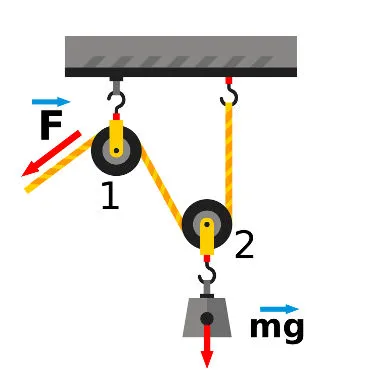
\includegraphics[width=.2\textwidth]{../../figuras/roldana.png}
		}
		\hfill
		\subfigure[calculadora]{
			 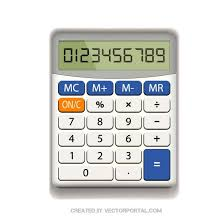
\includegraphics[width=.2\textwidth]{../../figuras/calculator.png}
		}
		\hfill
		\subfigure[computador]{
			 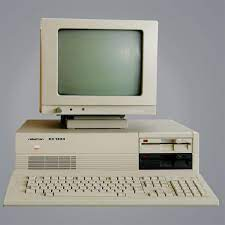
\includegraphics[width=.2\textwidth]{../../figuras/computer.png}
		}		  
		\caption{Criações humana.}
		\label{fig:figures}
	\end{figure}
\end{frame}




\begin{frame}
	\frametitle{Conceitos Fundamentais}
	\textbf{Motivação}
	\begin{itemize}
		\item Um \textbf{computador}:
		\begin{itemize}
			\item rápido e preciso, mas é uma máquina dependentes. Não tem iniciativa, não é criativos nem inteligente.
			\item precisa de instruções detalhadas para realizar uma tarefa
			\item tem por finalidade receber, manipular e armazenar dados, num ciclo de entrada-processamento-saída)
			\item é formado por \textit{hardware} e \textit{software}
		\end{itemize}
	\end{itemize}


	\begin{figure}
		\centering
		\subfigure[\textit{hardaware}] {
			 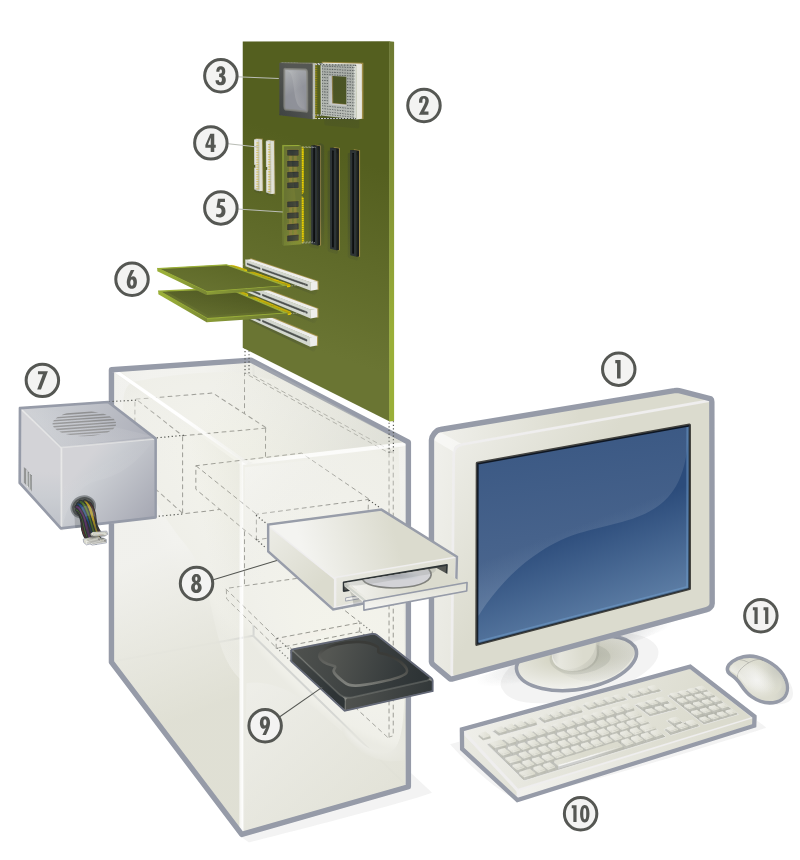
\includegraphics[width=.2\textwidth]{../../figuras/hardware.png}
		}
		\subfigure[\textit{software}]{
			 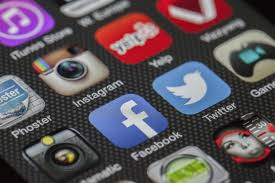
\includegraphics[width=.2\textwidth]{../../figuras/softwares.png}
		}
		\caption{Partes de um computador.}
		\label{fig:hardaware-software}
	\end{figure}
\end{frame}



\begin{frame}
	\frametitle{Conceitos Fundamentais}
	\textbf{Motivação}
	\begin{itemize}
		\item Para um computador realizar uma determinada tarefa, devemos escrever um programa ou vários programas interconectados.
		\item Para que o computador execute o programa, devemos escrevê-lo em uma linguagem que o computador e a pessoa que está escrevedo compreendam as instruções.
		\item Esse tipo de linguagem é chamada de \textbf{Linguagem de Programação}.
	\end{itemize}

	\begin{figure}
		\centering
		
\includegraphics[width=.4\textwidth]{../../figuras/languages.png}
		
		\caption{Algumas Linguagens de Programação.}
		\label{fig:languages}
	\end{figure}
\end{frame}


\section{Programação}
\begin{frame}
	\frametitle{Programação}
	\textbf{Introdução}
	\begin{itemize}
		\item \textbf{Programação} é o processo de criar um conjunto de instruções que dizem a um computador como realizar uma tarefa (\textbf{programa}). 
		\item Como desenvolver um programa?
		\begin{itemize}
			\item Análise do problema ou tarefa.
			\item Elaboração de um algoritmo.
			\item Codificação.
		\end{itemize}
	\end{itemize}
\end{frame}





\begin{frame}
	\frametitle{Programação}
	\framesubtitle{Etapas para desenvolver um programa}
	Etapa 1 - \textbf{Análise do problema ou tarefa}:
	\begin{itemize}
		\item estudar o enunciado do problema para entendê-lo ;
		\item definir quais e como são os dados de entrada (estrutura)
		\item definir como será o processamento (cálculos e atribuições de valor)
		\item definir os dados de saída 
	\end{itemize}
\end{frame}


\begin{frame}
	\frametitle{Programação}
	\framesubtitle{Etapas para desenvolver um programa}
	Etapa 2 - \textbf{Elaboração de um algoritmo}:
	\begin{itemize}
		\item pensar em uma solução para o problema estudado.
		\item técnicas para representação:
		\begin{itemize}
			\item \textbf{Descrição Narrativa}
			
			\item \textbf{Fluxograma}
			
			\item \textbf{Pseudocódigo}	
		\end{itemize}
	
	\end{itemize}
	
\end{frame}


\begin{frame}
	\frametitle{Programação}
	\framesubtitle{Etapas para desenvolver um programa}
	Etapa 3 - \textbf{Codificação}:
	\begin{itemize}
		\item transformar o algoritmo elaborado na Etapa 2 em um programa (códigos) utilizando uma linguagem de programação.
	\end{itemize}
\end{frame}



\begin{frame}
	\frametitle{Programação}
	\framesubtitle{Etapas para desenvolver um programa}
	\textbf{Resumo}

	\begin{figure}
		\centering
		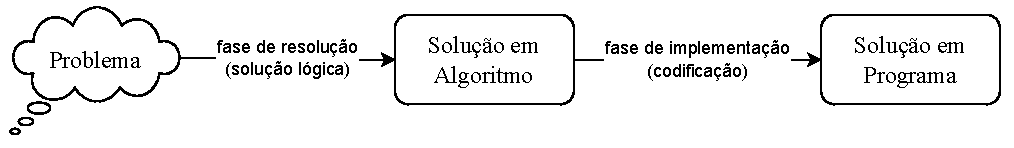
\includegraphics[width=0.9\textwidth]{../../figuras/etapas-programacao.pdf}\\[-2ex]
		\caption{Etapas da programação.}
		\label{fig:etapas-programacao-2}
	\end{figure}
\end{frame}

